\documentclass[../Main.tex]{subfiles}

\begin{document}

\IfFileExists{NewCommands.tex}       {% Add new commands here.
%
% Use "providecommand" instead of "newcommand" since we
% want to include this file in all subfiles, and if we
% used newcommand it would report the error
% "Command xxx already defined"
%
%
\providecommand{\dmOT}{\Delta m^2_{\rm 12}}
\providecommand{\dmsolar}{\Delta m^2_{\rm solar}}
\providecommand{\dmatm}{\Delta m^2_{\rm atm}}
\providecommand{\dmTT}{\Delta m^2_{\rm atm}}
\providecommand{\dmsq}[1]{\Delta m^{2}_{#1}}
\providecommand{\thatm}{\Delta m^2_{\rm atm}}
\providecommand{\thTT}{\theta_{\rm 23}}
\providecommand{\sinsq}[1]{\sin^{2}(\theta_{#1})}
\providecommand{\sinsqOT}{\sin^{2}(\theta_{\rm 12})}
\providecommand{\sinsqsolar}{\sin^{2}(\theta_{\rm solar})}
\providecommand{\sinsqTT}{\sin^{2}(\theta_{\rm 23})}
\providecommand{\sinsqTwoTT}{\sin^{2}(2\theta_{\rm 23})}
\providecommand{\dcp}{\delta_{\rm CP}}

\providecommand{\gsim}{\gtrsim}
\providecommand{\lsim}{\lesssim}
\providecommand{\Enu}{\rm{E}_\nu}
\providecommand{\Emu}{\rm{E}_\mu}
\providecommand{\Ecasc}{\rm{E}_{\rm casc}}
\providecommand{\Lmu}{\rm{L}_\mu}
\providecommand{\Lnu}{\rm{L}_\nu}
\providecommand{\Thetamu}{\theta_\mu}
\providecommand{\cosThetamu}{\cos{\theta_\mu}}
\providecommand{\cosThetanu}{\cos{\theta_\nu}}
\providecommand{\Thetanu}{\theta_\nu}
\providecommand{\nue}{\nu_{\rm e}}
\providecommand{\numu}{\nu_\mu}
\providecommand{\nutau}{\nu_\tau}

\providecommand{\ket}[1]{|#1\rangle}

\providecommand{\ue}[1]{|U_{e #1}|}
\providecommand{\umu}[1]{|U_{\mu #1}|}
\providecommand{\utau}[1]{|U_{\tau #1}|}
\providecommand{\uesq}[1]{|U_{e #1}|^{2}}
\providecommand{\umusq}[1]{|U_{\mu #1}|^{2}}
\providecommand{\utausq}[1]{|U_{\tau #1}|^{2}}

\providecommand{\Nch}{${\rm N}_{\rm ch}\,$}
\providecommand{\Ndir}{${\rm N}_{\rm dir}\,$}
\providecommand{\Nstr}{${\rm N}_{\rm str}\,$}
\providecommand{\Aeff}{${\rm A}_{\rm eff}\,$}
\providecommand{\Veff}{${\rm V}_{\rm eff}\,$}
\providecommand{\VeffNS}{${\rm V}_{\rm eff}$}

\providecommand{\pe}{$p.e.$ }
}       {}
\IfFileExists{../NewCommands.tex}    {% Add new commands here.
%
% Use "providecommand" instead of "newcommand" since we
% want to include this file in all subfiles, and if we
% used newcommand it would report the error
% "Command xxx already defined"
%
%
\providecommand{\dmOT}{\Delta m^2_{\rm 12}}
\providecommand{\dmsolar}{\Delta m^2_{\rm solar}}
\providecommand{\dmatm}{\Delta m^2_{\rm atm}}
\providecommand{\dmTT}{\Delta m^2_{\rm atm}}
\providecommand{\dmsq}[1]{\Delta m^{2}_{#1}}
\providecommand{\thatm}{\Delta m^2_{\rm atm}}
\providecommand{\thTT}{\theta_{\rm 23}}
\providecommand{\sinsq}[1]{\sin^{2}(\theta_{#1})}
\providecommand{\sinsqOT}{\sin^{2}(\theta_{\rm 12})}
\providecommand{\sinsqsolar}{\sin^{2}(\theta_{\rm solar})}
\providecommand{\sinsqTT}{\sin^{2}(\theta_{\rm 23})}
\providecommand{\sinsqTwoTT}{\sin^{2}(2\theta_{\rm 23})}
\providecommand{\dcp}{\delta_{\rm CP}}

\providecommand{\gsim}{\gtrsim}
\providecommand{\lsim}{\lesssim}
\providecommand{\Enu}{\rm{E}_\nu}
\providecommand{\Emu}{\rm{E}_\mu}
\providecommand{\Ecasc}{\rm{E}_{\rm casc}}
\providecommand{\Lmu}{\rm{L}_\mu}
\providecommand{\Lnu}{\rm{L}_\nu}
\providecommand{\Thetamu}{\theta_\mu}
\providecommand{\cosThetamu}{\cos{\theta_\mu}}
\providecommand{\cosThetanu}{\cos{\theta_\nu}}
\providecommand{\Thetanu}{\theta_\nu}
\providecommand{\nue}{\nu_{\rm e}}
\providecommand{\numu}{\nu_\mu}
\providecommand{\nutau}{\nu_\tau}

\providecommand{\ket}[1]{|#1\rangle}

\providecommand{\ue}[1]{|U_{e #1}|}
\providecommand{\umu}[1]{|U_{\mu #1}|}
\providecommand{\utau}[1]{|U_{\tau #1}|}
\providecommand{\uesq}[1]{|U_{e #1}|^{2}}
\providecommand{\umusq}[1]{|U_{\mu #1}|^{2}}
\providecommand{\utausq}[1]{|U_{\tau #1}|^{2}}

\providecommand{\Nch}{${\rm N}_{\rm ch}\,$}
\providecommand{\Ndir}{${\rm N}_{\rm dir}\,$}
\providecommand{\Nstr}{${\rm N}_{\rm str}\,$}
\providecommand{\Aeff}{${\rm A}_{\rm eff}\,$}
\providecommand{\Veff}{${\rm V}_{\rm eff}\,$}
\providecommand{\VeffNS}{${\rm V}_{\rm eff}$}

\providecommand{\pe}{$p.e.$ }
}    {}
\IfFileExists{../../NewCommands.tex} {% Add new commands here.
%
% Use "providecommand" instead of "newcommand" since we
% want to include this file in all subfiles, and if we
% used newcommand it would report the error
% "Command xxx already defined"
%
%
\providecommand{\dmOT}{\Delta m^2_{\rm 12}}
\providecommand{\dmsolar}{\Delta m^2_{\rm solar}}
\providecommand{\dmatm}{\Delta m^2_{\rm atm}}
\providecommand{\dmTT}{\Delta m^2_{\rm atm}}
\providecommand{\dmsq}[1]{\Delta m^{2}_{#1}}
\providecommand{\thatm}{\Delta m^2_{\rm atm}}
\providecommand{\thTT}{\theta_{\rm 23}}
\providecommand{\sinsq}[1]{\sin^{2}(\theta_{#1})}
\providecommand{\sinsqOT}{\sin^{2}(\theta_{\rm 12})}
\providecommand{\sinsqsolar}{\sin^{2}(\theta_{\rm solar})}
\providecommand{\sinsqTT}{\sin^{2}(\theta_{\rm 23})}
\providecommand{\sinsqTwoTT}{\sin^{2}(2\theta_{\rm 23})}
\providecommand{\dcp}{\delta_{\rm CP}}

\providecommand{\gsim}{\gtrsim}
\providecommand{\lsim}{\lesssim}
\providecommand{\Enu}{\rm{E}_\nu}
\providecommand{\Emu}{\rm{E}_\mu}
\providecommand{\Ecasc}{\rm{E}_{\rm casc}}
\providecommand{\Lmu}{\rm{L}_\mu}
\providecommand{\Lnu}{\rm{L}_\nu}
\providecommand{\Thetamu}{\theta_\mu}
\providecommand{\cosThetamu}{\cos{\theta_\mu}}
\providecommand{\cosThetanu}{\cos{\theta_\nu}}
\providecommand{\Thetanu}{\theta_\nu}
\providecommand{\nue}{\nu_{\rm e}}
\providecommand{\numu}{\nu_\mu}
\providecommand{\nutau}{\nu_\tau}

\providecommand{\ket}[1]{|#1\rangle}

\providecommand{\ue}[1]{|U_{e #1}|}
\providecommand{\umu}[1]{|U_{\mu #1}|}
\providecommand{\utau}[1]{|U_{\tau #1}|}
\providecommand{\uesq}[1]{|U_{e #1}|^{2}}
\providecommand{\umusq}[1]{|U_{\mu #1}|^{2}}
\providecommand{\utausq}[1]{|U_{\tau #1}|^{2}}

\providecommand{\Nch}{${\rm N}_{\rm ch}\,$}
\providecommand{\Ndir}{${\rm N}_{\rm dir}\,$}
\providecommand{\Nstr}{${\rm N}_{\rm str}\,$}
\providecommand{\Aeff}{${\rm A}_{\rm eff}\,$}
\providecommand{\Veff}{${\rm V}_{\rm eff}\,$}
\providecommand{\VeffNS}{${\rm V}_{\rm eff}$}

\providecommand{\pe}{$p.e.$ }
} {}


\graphicspath{{figures/}{Detector/figures/}}



\section{The detector: IceCube DeepCore}
\label{sec:detector}
The IceCube Neutrino Observatory \cite{icecube} is an ice Cherenkov neutrino telescope, buried 1.5\,km deep in the Antarctic ice at the geographic South Pole (see Fig.\,\ref{fig:ICFigure}). The detector consists of 5\,160 light sensors distributed over a volume of a cubic kilometer, which monitor the ice permanently. At the surface it has an array of ice filled tanks that detect cosmic rays via air showers, named IceTop.

The main goal of IceCube is the detection of neutrinos emitted outside the solar system. Atmospheric neutrinos are a source of background for this kind of search, as well as a potential signal for others. In order to use atmospheric neutrinos the detector was more densely instrumented towards its bottom using more efficient sensors. This allows the instrument to detect neutrino interactions of lower energies in this particular volume. The subarray is called DeepCore \cite{dcdesign}.

\begin{figure}[bth]
  \centering
  \hspace*{\fill}
  \begin{subfigure}[c]{0.48\textwidth}
    \centering
    \includegraphics[width=\textwidth]{IceCubeNoLabels}
    \caption{Schematic view}
    \label{fig:ICdiagram}
  \end{subfigure}
  \begin{subfigure}[c]{0.5\textwidth}
    \centering
    \includegraphics[width=\textwidth]{DOM}
    \caption{Digital Optical Module}
    \label{fig:DOM}
  \end{subfigure}
  \caption[The IceCube Neutrino Observatory.]{The IceCube Neutrino Observatory and its detection unit.}
  \label{fig:ICFigure}
\end{figure}

\subsection{Principle of operation}
\label{sec:icoperation}
Charged particles traversing a medium faster than the local speed of light emit electromagnetic radiation, a phenomenon known as the Cherenkov effect (discussed in Sec.\,\ref{sec:cherenkov}). The operation of IceCube relies entirely on the detection of these photons, together with their arrival time and the position of the sensor that records them.

The photons are recorded by individual detection units, known as Digital Optical Modules (DOMs). The main components of a DOM are a 10'' Hamamatsu photomultiplier (PMT), a mainboard with the necessary electronics to supply power and digitize the signal, an array of light emitting diodes and a 13'' glass sphere, which encloses all of the above \cite{DOMdesign}.

The detection of a photon starts when it arrives at the DOM and crosses the 0.5'' thick glass sphere. Leaving the sphere it enters a gel which is used to optically couple the sphere and the PMT. Once in the PMT, the photon can be absorbed by a photocathode, emitting an electron which is then amplified. The resulting signal is readout as a change in the voltage of the PMTs anode, and given to the mainboard electronics.

The voltage at the PMTs anode is fed to three pieces of circuitry, one for triggering and two more for reading out the signal in high and low resolution modes. The high resolution readout path consists of two custom 10-bit analog-to-digital converters, known as ATWDs, operated at 300 mega samples per second (MSPS). An ATWD has 3 input channels at different amplification levels, and capture results in the recording of 128 analog samples at each one of them. A signal is readout with a maximum duration of 426\,ns and a bin size of about 3.3\,ns \cite{icecube_pmt}. For signals that might take a longer time to develop, a low resolution converter (fADC) is available. The fADC is operated at 40 MSPS, and capture consists of 256 samples, which cover an interval of a little over 6\,$\mu$s with a bin size of 25\,ns \cite{DAQ}.

When a DOM records a signal with an integrated charge above the 0.25\,PE threshold it communicates with its nearest and next-to-nearest neighbors to determine if any of these DOMs have also crossed the threshold. The allowed time interval is $\pm1$ $\mu$s. This search is repeated for each DOM that is found above threshold. When two or more DOMs fulfill the criteria, they are given the ``Hard Local Coincidence'' (HLC) tag, and are readout both in high and low resolution modes. Modules above the threshold but without an HLC tag are readout in low resolution mode only. A summarized comparison between the two readout modes with their respective conditions can be found in Table \ref{table:DOMreadout}.

\begin{table}[h]
\caption[Readout modes of the IceCube DOMs.]{Readout modes of the IceCube Digital Optical Modules. From \cite{DAQ}.}
\label{table:DOMreadout}
\centering
\begin{Tabular}[1.]{lcccc}
\hline
Readout path & Condition & Sampling rate & Capture & Resolution \\
\hline
ATWD  & HLC & 300 MSPS & 128 samples  & 3\,ns\\
fADC & Above threshold & 40 MSPS & 256 samples & 25\,ns\\
\hline
\end{Tabular}
\end{table}

The output of reading out a DOM is a digitized waveform. An unfolding procedure is conducted to determine the time at which the signal appeared, its duration, and the number of photons that created it. Given the finite time and voltage resolutions, individual photons cannot always be discerned. Instead, the concept of \textit{pulses} is introduced. A pulse describes the charge $Q$ deposited in the DOM by a bundle of photons during a time interval $t + \Delta t$. The time interval can vary according to the results from the unfolding, but is typically of the order of the resolution of the capture method used. This means that multiple pulses can appear in one DOM during one event, which lasts for several microseconds. The charge is normalized to the single photon case, and expressed in units of photoelectrons (PEs). These two quantities, charge $Q$ and time $t$, are the detector's observables which are available for analysis.

\subsection{Detector layout}
\label{sec:fv}
The DOMs are arranged in strings. Each string supports 60 DOMs and there are 86 of them. The 80 ``standard'' IceCube strings are instrumented from a depth of 1\,450\,m to 2\,450\,m, with a spacing of 17\,m between sensors. The layout of the strings follows a concentric hexagonal pattern, with a typical distance of 125\,m to the nearest neighbor, as it can be seen in Fig.\,\ref{fig:ICgeometry} \cite{icecube}.

In addition there are 8 dedicated DeepCore strings, which use PMTs with 35\,\% higher quantum efficiency with respect to the standard ones. Six of these surround the central IceCube string. They follow the same hexagonal pattern with a smaller separation, of 70\,m. The two remaining strings are deployed inside the DeepCore region. DOMs on DeepCore strings are 7\,m apart and only start at a depth of 1.75\,km, with a large gap between the positions of the 10th and 11th DOM (see Fig.\,\ref{fig:ICsideview}) \cite{dcdesign}. 

The DeepCore fiducial volume, as is used later on in the data analysis, is defined in the $x-y$ plane by the DeepCore strings, the central string, and the first hexagon of standard IceCube strings (see Fig.\,\ref{fig:ICgeometry}). In the $z$ direction, the volume starts at a depth of 2\,100\,m. Standard IceCube strings have 18 DOMs below this depth; DeepCore strings have 50. Figure \ref{fig:ICsideview} is a sketch of the side projection of the detector and the fiducial volume.

\begin{figure}[bth]
  \begin{subfigure}[c]{0.49\textwidth}
    \centering
    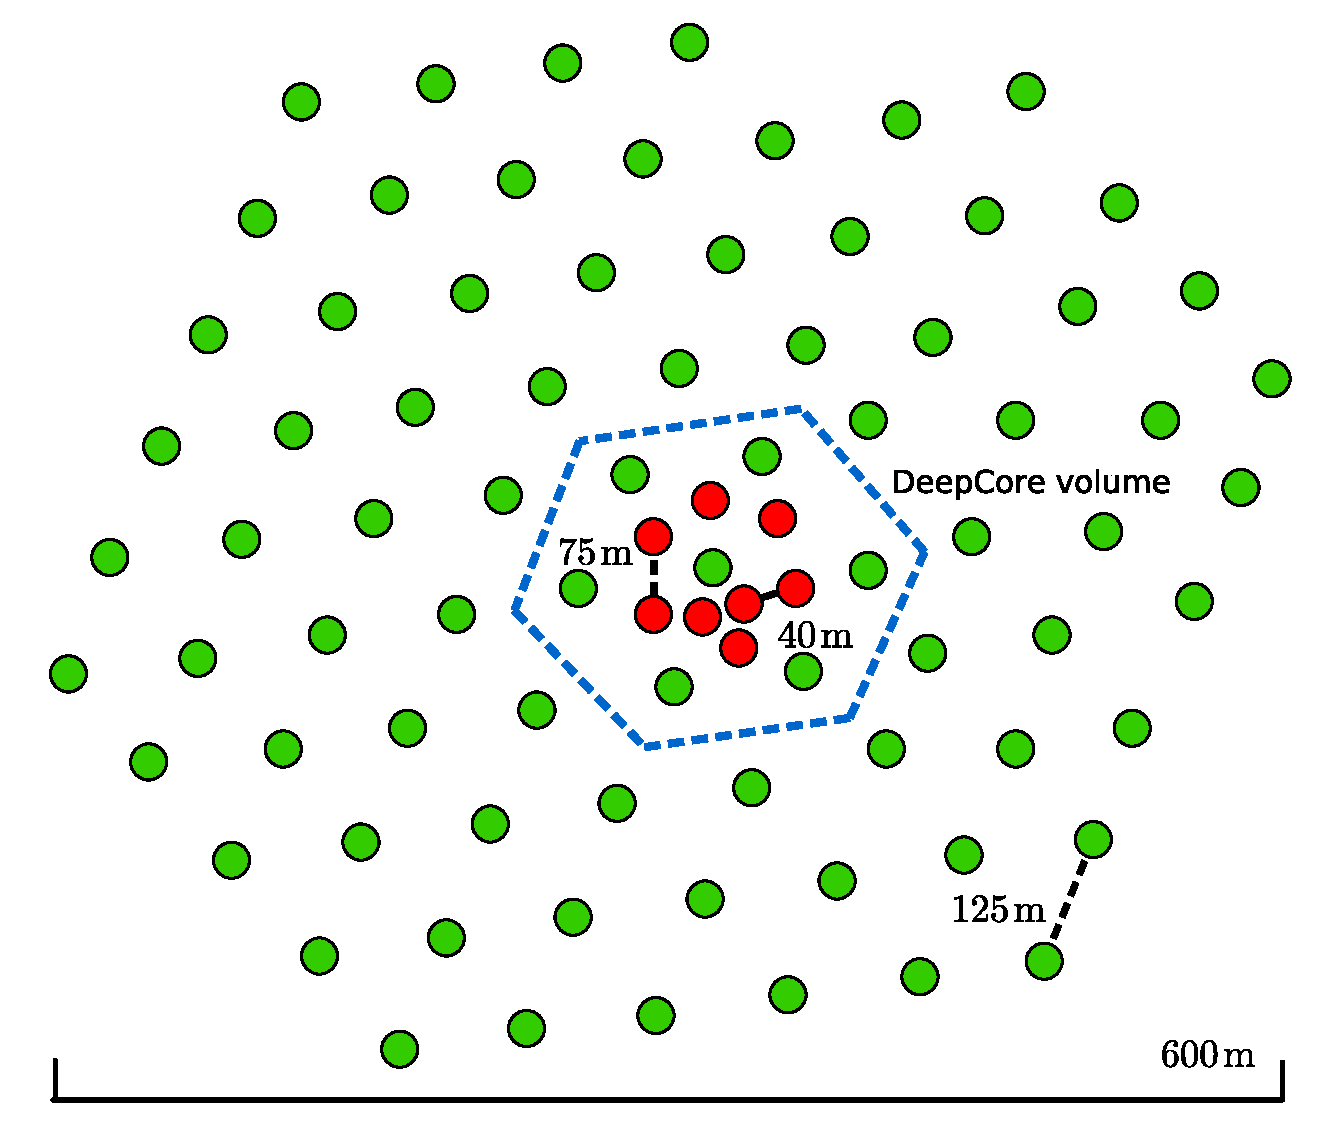
\includegraphics[width=\textwidth]{Geometry}
    \caption{Footprint view}
    \label{fig:ICgeometry}
  \end{subfigure}
  \hfill
  \begin{subfigure}[c]{0.49\textwidth}
    \centering
    \includegraphics[width=\textwidth]{DeepCoreNew}
    \caption{Side view}
    \label{fig:ICsideview}
  \end{subfigure}
  \caption[Schematic projections of the IceCube detector.]{Top and lateral projections of the IceCube detector. The DeepCore fiducial volume is marked in blue (a) and green (b). Panel (b) taken from \cite{deepcore_capabilities}.}
  \label{fig:ICschematic}
\end{figure}


\subsection{Detection medium}
\label{sec:DetectionMedium}
The ice of the Antarctic glacier was formed from snow after it was compacted under its own weight in a very slow process. The result of this process is a layered structure, with an air bubble content that decreases with depth. The clearest ice starts at depths of around 1.4\,km. There the medium has a transparency that is not possible to match in laboratory conditions \cite{ice1}.

The optical properties of the ice, i.e. scattering and absorption, affect the trajectory of the light produced by charged particles. These properties are studied by using data taken by a ``dust logger'' device, and also with data acquired by the experiment itself while operating in LED flashing mode. The data are fit by assuming that optical properties change with depth, but are constant in the $x-y$ plane. Figure \ref{fig:IceProperties} shows the result from two such fits, for light of 400\,nm of wavelength. The absorption coefficient, shown in the left panel, is defined as the average distance traveled by a photon before it is absorbed. The geometrical scattering $b$, which determines the average distance between successive scatters as $1/b$, is used to define an effective scattering coefficient $b_e = b\cdot (1-\left<\cos\theta\right>)$, where $\theta$ is the deflection angle at each scatter point \cite{ice2}.

The most striking feature is the existence of a region at a depth of about 2.1\,km with abnormal values. The reason for this is an unusually high accumulation of dust; the existence of this layer was also observed by the dust logger. Aside from the dust layer it can also be seen that the ice has a complicated small scale structure, with absorption and scattering coefficients that vary as much as 30\,\% from their mean values.
% http://www.astro.wisc.edu/~heroux/history.html, search for amanda paper?

\begin{figure}[bth]
  \centering
  \begin{subfigure}[c]{0.49\textwidth}
    \centering
    \includegraphics[width=0.95\textwidth]{IceAbsorption}
    \caption{Absorption}
    \label{fig:IceAbsorption}
  \end{subfigure}
  \begin{subfigure}[c]{0.49\textwidth}
    \centering
    \includegraphics[width=0.95\textwidth]{IceScattering}
    \caption{Scattering}
    \label{fig:IceScattering}
  \end{subfigure}
  \caption[Optical properties of the South Pole ice.]{Optical properties of the South Pole ice inferred from two different studies. From \cite{ice2}.}
  \label{fig:IceProperties}
\end{figure}

Apart from the compacted ice, the photons travel through a second kind of ice structure before reaching the DOMs. The construction of IceCube required drilling holes and melting columns of ice to deploy the instrumentation. The refreezing of the water in the holes left ice columns with optical properties rather different from those of the bulk of the ice. This \textit{borehole ice} is modeled by assuming a dense concentration of bubbles, with the best fit given by a scattering length of 50\,cm. This can be compared with the effective scattering length from Fig.\,\ref{fig:IceScattering}, which in the dust layer is of about 5\,m.



\textbf{[NOTES: have to describe HLC, SLC, and at least pulses. Probably have
  to include DOMLaunch description because we used those in the filter
  and in IC79 and in some other places too.]}

\end{document}
